Technically, no official definition of nonlinear time series, but sometimes, there is an obvious choice for what to call linear or nonlinear. \\

For time series like \[X_t = f(X_{t-1} ... X_{t-p}) + \varepsilon_t \]
\begin{itemize}
    \item if $f(X_{t-1} ... X_{t-p})$ is something like $ =\alpha_1 X_{t-1} + ...+ \alpha_p X_{t-p}$ call this linear. Otherwise, nonlinear.
\end{itemize}
ARMA models are considered linear by everyone. 

\subsection{Why non-linearity?}

\begin{figure}[H]
\centering
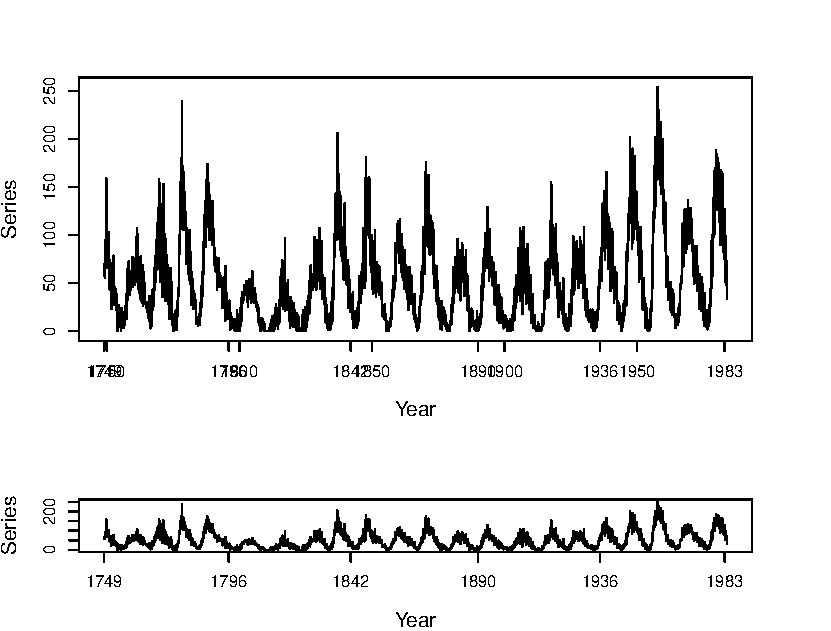
\includegraphics[scale=0.8]{plots/sunpots.pdf}
\caption{Average monthly sunspot numbers from 1860 to 1983. The lower graph has a shortened vertical axis, which enables the rise and fall of the graph to be more easily assessed.}
\end{figure}

Graph shows there is regular cyclic behavior with a period of approximately 11 years. But we also see that the series generally increases at a faster rate than it decreases. \textbf{Behavior like this cannot be explained by a linear model}.\
"Such asymmetric behavior can also arise in studying the economy since the relationship between economic variables tend to be different when the economy is moving into recession rather than when coming out of one" (p.268). \\

"For seasonal series with a fixed cycle length, it may be possible to model asymmetric behavior with a non-sinusoidal seasonal component, but when the cycle length is not fixed, a non-linear model is much more compelling for describing series with properties such as 'going up faster than coming down'" (p.269).\\

Before starting non-linear analysis, it is sensible to ensure that the data really is non-linear. But tests for non-linearity often have poor power, and the simplest, and arguably the most important tool is a careful inspection of the time plot. 


\subsection{Threshold AR models}
A \textbf{threshold AR (TAR) model} is a piecewise linear model where the parameters of an AR model are determined by the values by the values taken by one or more of the lagged values of the time series. \\

Idea: Glue together two different AR models.\\

Simplest way is depending on value of $X_{t-1}$:
\begin{subequations}
\begin{empheq}[left = {X_t=\empheqlbrace}]{align*} 
    &v_1 + a_1X_{t-1} + \sigma_1 \varepsilon_t &&\text{if $X_{t-1} < r$} \\
    &v_2 + a_2 X_{t-1} + \sigma_2 \varepsilon_t &&\text{if $X_{t-1}\geq r$}
\end{empheq}
\end{subequations}
The AR parameter depends on whether $X_{t-1}$ exceeds the value $r$, called the \textbf{threshold}.


\begin{figure}[h]
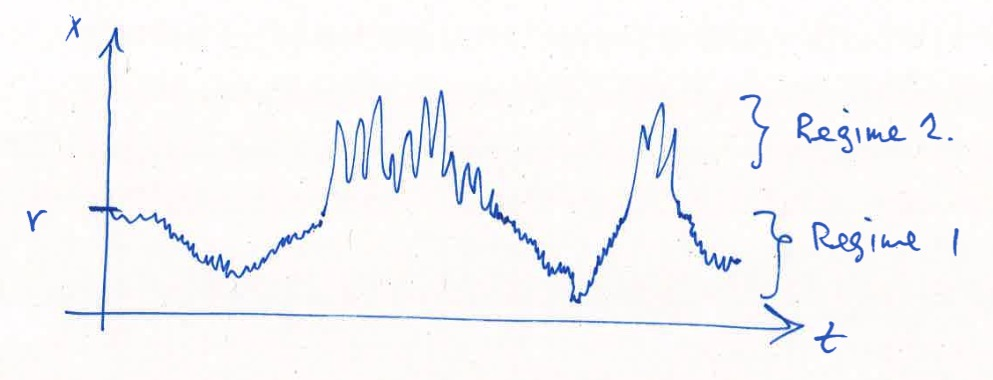
\includegraphics[scale=0.4]{images/Screenshot 2024-05-06 at 08.49.15.jpg}
\centering
\end{figure}


Estimation: Choose a distribution for $\varepsilon_t$ (like $N(0,1)$) and do maximum likelihood. \[\rightarrow \hat{v}_1,\hat{v}_2,\hat{\alpha}, \hat{\alpha}_2, \hat{\sigma}_1, \hat{\sigma}_2, \hat{r}  \]

\subsection{Volatility Models}

Whereas the previous non-linear model allow for improved point forecasts of the observed variable to be made when the true model is known, we here focus on \textbf{volatility models} that are primarily concerned with modelling \textit{changes in variance} or \textit{volatility}. They do not generally lead to better point forecasts, but may lead to better estimates of the (local) variance. This, in turn, allows more reliable prediction intervals and hence a better assessment of risk. 

\begin{figure}[H]
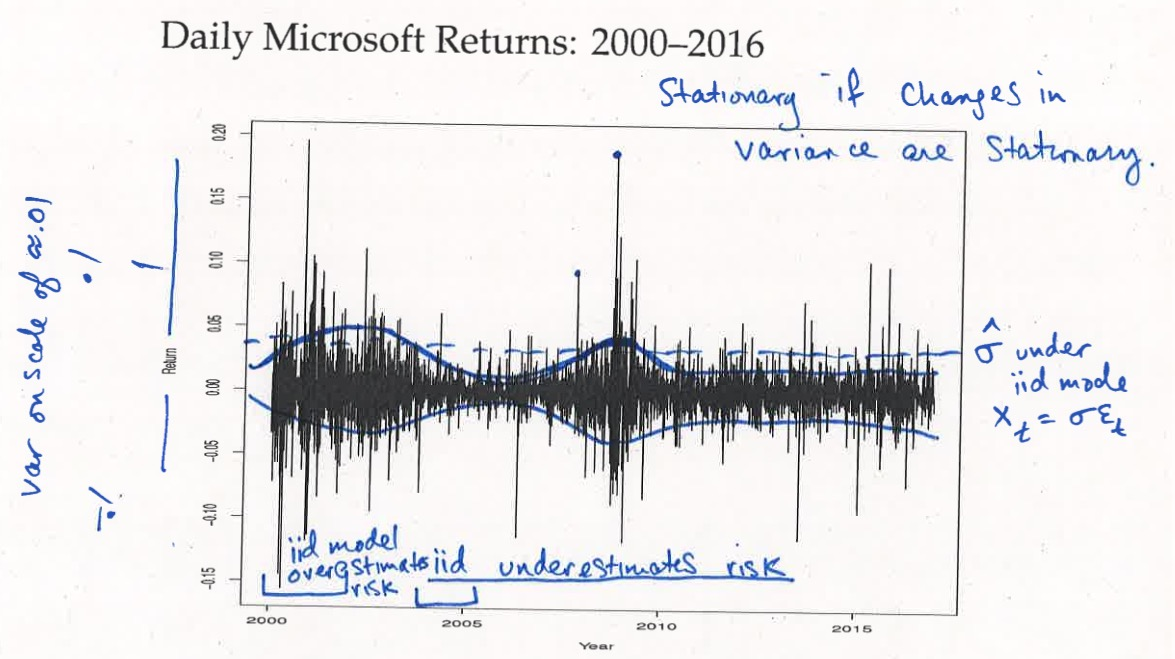
\includegraphics[scale=0.4]{images/Screenshot 2024-05-13 at 09.11.00.jpg}
\centering
\end{figure}


There are swells in the variance of the time series. \\
ARMA models cannot capture this behavior. \\

Suppose: try modeling Daily Microsoft returns with a fixed variance model.
\begin{itemize}
    \item Might use efficient markets: $E[X_t]=0$
    \item That leaves \[
    X_t =\sigma \cdot \varepsilon_t \quad \text{with $\varepsilon_t$ iid. and $var(\varepsilon_t)=1$.}
    \]
    \item What if someone asks: "How much risk is there in microsoft returns tomorrow?
    \begin{itemize}
        \item Observe $X_t \quad t=1,...,T$
        \item Question is about $var(X_{T+1})$ essentially. Might start by asking, what is an estimate $\hat{var}(X_{T+1})$
        \item But if you estimate $\hat{\sigma}$ in a model $X_t=\sigma \varepsilon_t$ \begin{itemize}
            \item Then $\hat{Var}(x_{T+1})=\hat{\sigma}^2$ regardless of $T$ or recent history.
        \end{itemize}
    \end{itemize}
\end{itemize}


\subsubsection{ARCH Models}
\underline{A}uto\underline{r}egressive \underline{C}onditional \underline{H}eteroskedasticity \quad [first-order case]

\[X_t= \sigma_t \varepsilon_t\]
\begin{itemize}
    \item $\varepsilon_t$ mean-zero, purely random (iid.) process with $var(\varepsilon_t)=1$
    \item $\sigma_t^2=\gamma +\alpha X_{t-1}^2$ \quad (the variance depends on the most recent value of the derived series) 
    \begin{itemize}
        \item $\sigma_t^2 = \gamma + \sum_{j=1}^k \alpha_j X_{t-j}^2$ [General form]
    \end{itemize}
\end{itemize}

\noindent 
Comments: 
\begin{itemize}
    \item oddly named, because $\sigma_t^2$ "regressed" on past $X_{t-1}$ rather than $\sigma_{t-1}^2$
    \item Compactly written $X_t=\sqrt{\gamma+ \alpha X_{t-1}^2}\varepsilon_t$
    \item There is no error term in $\sigma_t^2$ equation.
    \item Unconditional mean is zero: $E(X_t)=E(E(X_t|F_{t-1})) = E(\sigma_t E(\varepsilon_t))=0 $
\begin{itemize}
    \item Derivation:
\end{itemize}
    \begin{align*}
        Var(X_t)&=E(X_t^2) = E(\gamma + \alpha X_{t-1}^2) = \gamma + \alpha E(X_{t-1}^2) \\
        \text{As $X_t$ is stationary: } Var(X_t)&=Var(X_{t-1})=E(X_{t-1}^2) \\
        \Rightarrow Var(X_t)&= \gamma + \alpha Var(X_t) \\
        1&= \frac{\gamma}{Var(X_t)} + \alpha \\
        Var(X_t)&=\frac{\gamma}{1-\alpha}
    \end{align*}
    \item The process is stationary (extended infinitely forward and backward)
    \[var(X_t)=\frac{\gamma}{1-\alpha} \quad \text{(unconditional variance)}\]
    \item If $\alpha>0$, large $X_{t-1}^2 \Rightarrow$ large $\sigma_t^2$
    \begin{itemize}
        \item[] $\Rightarrow$ average $\sigma_t^2$ is larger than if $\alpha=0$ were true
        \item[] $\Rightarrow$ Larger conditional variance 
    \end{itemize}
    \item Example: $\alpha=\frac{1}{2} \Rightarrow var(X_t)=\frac{\gamma}{1-\frac{1}{2}} = 2\gamma> \gamma$ 
\end{itemize}
One nice property of ARCH models is that the tail distribution of $X_t$ is heavier than that of a normal distribution. Hence the innovation process $X_t$ in a Gaussian ARCH(1) model tends to generate more 'outliers' than a Gaussian white noise process.\\

\noindent
Parameters in ARCH models can be estimated by maximizing their likelihood. \\

\noindent
\underline{Book (not covered in lecture)} \\
\noindent
Consider an ARCH($k$) model. At forecast origin $N$, the 1-step-ahead forecast for $\sigma_{N+1}^2$ is \[
\sigma_N^2 (1)=E(\sigma_{N+1}^2| \mathcal{F}_N) = \gamma + \alpha_1 X_N^2 + \cdots + \alpha_k X_{N+1-k}^2
\]
and the $l$-step-ahead forecast for $\sigma_{N+l}^2$ is \[
\hat{\sigma}_N^2(l)= E(\sigma_{N+l}^2| \mathcal{F}_N) = \gamma + \sum_{i=1}^k \alpha_i \hat{\sigma}_N^2 (l-k)
\]

\subsubsection{GARCH Models}
The ARCH model has been generalized to allow the variance to depend on the past values of $\sigma_t^2$ as well as on past values of $X_t^2$.

Limitation of ARCH is $\sigma_t^2$ process resets if $\varepsilon_t \approx0$. 

\[X_t=\sigma_t \varepsilon_t\]
\begin{itemize}
    \item ARCH: $\sigma_t^2=\gamma+\alpha X_{t-1}^2$
    \item GARCH: $\sigma_t^2= \gamma+\alpha X_{t-1}^2 + \beta \sigma_{t-1}^2 $
    \begin{itemize}
        \item[] ("Autoregressive" process in $X_{t-1}^2$ and $\sigma_{t-1}^2$)
        \item Generalized: $\sigma_t^2 =\gamma + \sum_{j=1}^h \beta_j \sigma_{t-j}^2 + \sum_{i=1}^k \alpha_i X_{t-i}^2$
    \end{itemize}
\end{itemize}

Note: Alternative approach is \[ARCH(p): \sigma_t^2 = \gamma +\alpha_1 X_{t-1}^2 + \alpha_2 X_{t-2}^2 + \cdots + \alpha_p X_{t-p}^2\]
\begin{itemize}
    \item[]$\Rightarrow$ makes it harder for $\sigma_t^2$ to reset because it would need many $\varepsilon_t\approx 0$ in a row
    \item One advantage of GARCH over ARCH(p) is less parameters ($3 < p+1$ if $p$ is large)
\end{itemize}

Invertibility and stationarity assumptions of ARMA models apply to GARCH models. 

\textbf{\underline{How to estimate?}}
\begin{itemize}
    \item Assume a distribution for $\varepsilon_t$ (usually $\varepsilon_t \sim N(0,1)$)
    \item Perform maximum likelihood estimation.
    \item Jargon: if you assume $\varepsilon_t \sim N(0,1)$ in estimation but you think $\varepsilon_t \sim $ something else (e.g. $\varepsilon_t \sim t_k$) then this procedure called "Quasi Maximum Likelihood"
\end{itemize}

\subsection{Non-linear Deterministic Models}
Can generate a fully random time series $X_t$ by: 
\begin{itemize}
    \item Choosing $X_1$, randomly
    \item Choosing $X_t=f(X_{t-1})$ for $t\geq 2$ and $f$ a fixed function.
\end{itemize}

Example:
\[
f(x)=k\cdot x\cdot (1-x)
\]
\begin{itemize}
    \item If $X_1 \sim Unif[0,1]$, then $X_2$ is random and $X_2=k\cdot X_1 \cdot (1-X_1)$
    \item What is the distribution of $x_2$?
\end{itemize}